\begin{frame}{Задача пяти внешних тел}
	\vfill % Верхняя пружина — держит дистанцию от заголовка
	\begin{tcolorbox}[
		colframe=DeepBlue!35,       % Тонкий приглушенный синий контур
		colback=DeepBlue!1!Ivory,    % Мягкий фон, плавно сливающийся с Ivory
		boxrule=0.5pt,               % Ультратонкая рамка
		arc=3pt,                     % Легкое скругление
		top=5pt, bottom=5pt, left=4pt, right=4pt,
		before=\vspace{2pt}, after=\vspace{4pt}
		]
		\centering
		$\displaystyle \vec{u}_i'' = G \sum_{j \neq i} \frac{m_j(\vec{u}_j - \vec{u}_i)}{|\vec{u}_j - \vec{u}_i|^3}$ \\[0.15cm]
		$\displaystyle T = [0, 10^6]$
	\end{tcolorbox}
	
	\vspace{0.15cm}
	
	\centering
	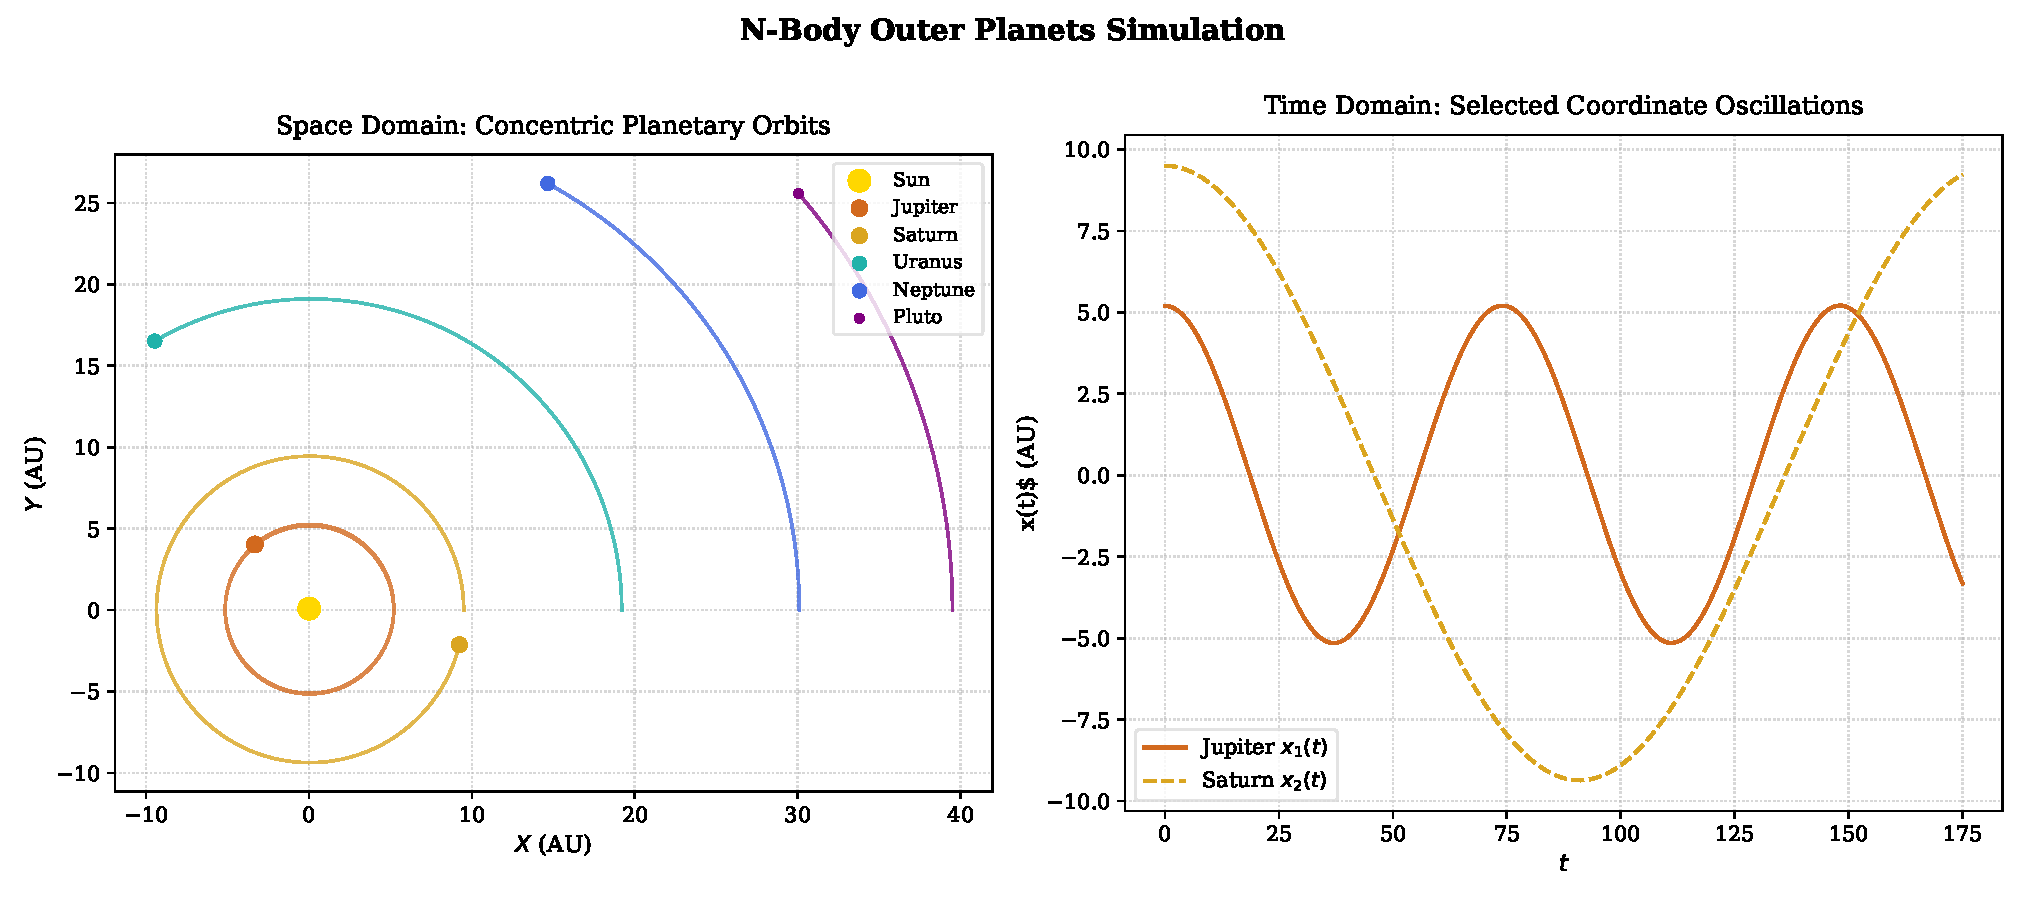
\includegraphics[height=0.5\textheight]{../code/results/visualization/nbody_planets_orbits}
	
	\vfill % Нижняя пружина — балансирует слайд над подвалом
\end{frame}